\section[toc=MB NCEL analysis]{The analysis of MB NCEL data}

%%%%% QEL FORMALISM %%%%%

\begin{slide}[toc = QEL formalism]{(Quasi-)elastic neutrino-nucleon scattering}
 
 \rput[c](13,4){% QEL vertex
\begin{pspicture}
  \rput[c](0,-1.75){Quasi-elastic scattering}
  \pscoil[coilarm = 0, linewidth = 0.025, linecolor = pdcolor1, coilwidth = 0.25, coilaspect = 0]{c-c}(-1,0)(1,0)
  \rput[c](0,-0.4){\color{pdcolor1}\small $W$}
  \psframe[linestyle = none, fillstyle = solid, fillcolor = pdcolor2](-1.1,-0.03)(-0.9,0.2)
  \psframe[linestyle = none, fillstyle = solid, fillcolor = pdcolor2](0.9,-0.03)(1.1,0.2)
  \pscircle[linestyle = none, fillstyle = solid, fillcolor = pdcolor1](-0.95,0){0.05}
  \pscircle[linestyle = none, fillstyle = solid, fillcolor = pdcolor1](0.95,0){0.05}
  \psline[linewidth = 0.025, linecolor = pdcolor1]{c-}(-0.95,0)(-2,1)
  \psline[linewidth = 0.025, linecolor = pdcolor1]{c-}(-0.95,0)(-2,-1)
  \psline[linewidth = 0.05, linecolor = pdcolor1]{c-}(0.95,0)(2,1)
  \psline[linewidth = 0.05, linecolor = pdcolor1]{c-}(0.95,0)(2,-1)
  
  \rput[l](-1.75,1){\color{pdcolor1} $l (k')$}
  \rput[l](-1.75,-1){\color{pdcolor1} $\nu (k)$}
  \rput[r](1.75,1){\color{pdcolor1} $p (p')$}
  \rput[r](1.75,-1){\color{pdcolor1} $n (p)$}

\end{pspicture}
}
 
 \begin{itemize}
  
  \item For (quasi-)elastic neutrino \\ scattering off nucleon \\ the cross section is given by:
  
  $$\hspace{-150pt}\sigma \sim \left|j_\mu h^{\mu}\right|^2$$

  \vspace{5pt}
  \item[$j_\mu$]$= \bar u(k')\gamma^\mu\left(1 - \gamma_5\right)u(k)$ $\rightarrow$ lepton current
  \item[$h_\mu$]$= \bar u(p')\Gamma^\mu u(p)$ \hspace{35pt} $\rightarrow$ hadron current
  \vspace{5pt}
  
  \item Leptonic vertex can be calculated from the basis.
  
  \item However, due to the complex structure of nucleon, hadronic vertex needs a phenomenological input.
  
  \item $\Gamma^\mu$ can be parametrized by the functions of $Q^2$, called form factors.
  
 \end{itemize}
 
\end{slide}

%%%%% FORM FACTORS %%%%%

\begin{wideslide}{Form factors}

 \begin{itemize}
    
  \item Hadronic vertex can be expressed in terms of form factors:
  
   $$\hspace{-60pt}\Gamma^\mu_{NC, p(n)} = \gamma^\mu {\color{pdcolor7}F_1^{NC, p(n)} (Q^2)} + \frac{i\sigma^{\mu\nu}q_\nu}{2M} {\color{pdcolor7}F_2^{NC, p(n)} (Q^2)} - \gamma^\mu\gamma_5 {\color{pdcolor6}G_A^{NC, p(n)} (Q^2)}$$
   
   \item Vector form factors are expressed by electromagnetic form factors {\it(Conserved Vector Current - CVC)}: 
 
    $$\hspace{-20pt}{\color{pdcolor7}F_{1,2}^{NC, p(n)}(Q^2)} = \pm\frac{1}{2}\left(F_{1,2}^p(Q^2) - F_{1,2}^n(Q^2)\right) - 2\sin^2\theta_WF_{1,2}^{p(n)}(Q^2) - \frac{1}{2}F_{1,2}^s(Q^2)$$
   
   \item Axial form factor is assumed to have a dipole form:
     
     $${\color{pdcolor6}G_A^{NC,p(n)}(Q^2)} = \pm\frac{1}{2}G_A(Q^2) - \frac{1}{2}G_A^s(Q^2) = (\pm g_A - \rnode{gs1}{g_A^s})\left(1 + Q^2 / \rnode{ma1}{M_A}^2\right)^{-2}$$
      
 \end{itemize}
 
 \rput[l](11,1.5){\color{pdcolor6} \rnode{ma2}{axial mass}}
 \rput[l](8,-0.25){\color{pdcolor6} \rnode{gs2}{strangeness}}
 
 \rput[c](1,-1)
 {
    \psframe[linewidth = 0.025, linecolor = pdcolor1](0,0)(5,1)
    \rput[c](2.5,0.75){\color{pdcolor1}\small different sign for proton/neutron}
    \rput[c](2.5,0.25){\color{pdcolor1}\small $g_A^s$ sensitive to $\sigma(\nu p) / \sigma(\nu n)$}
 }
 
 \psset{nodesep = 3pt}
 \ncarc[linecolor = pdcolor6]{->}{ma1}{ma2}
 \ncarc[linecolor = pdcolor6]{->}{gs1}{gs2}

\end{wideslide}

%%%%%% MB DATA %%%%%

\begin{slide}[toc=MiniBooNE data]{MiniBoonE data for NCEL}
  
  \onslide*{1}
  {
    \rput(12, 4.25)
    {
    \begin{pspicture}
    
      \pscircle[linestyle = none, fillstyle = solid, fillcolor = pdcolor1](0,0){1}

      \pscircle[linestyle = none, fillstyle = solid, fillcolor = pdcolor4](-2.5,0){0.2}
      \psline[linewidth = 0.05, linecolor = pdcolor4]{->}(-2.1,0)(-1.2,0)
      \rput[c](-1.7,0.2){\color{pdcolor4}\small $\nu_\mu$}
      \psline[linewidth = 0.05, linecolor = pdcolor1]{->}(1.2,0)(1.6,0)
      
      \rput[l](2,0.75){\color{pdcolor1} 0$\mu$}
      \rput[l](2,0){\color{pdcolor1} 0$\pi^\pm$}
      \rput[l](2,-0.75){\color{pdcolor1} 0$\pi^0$}
      
    \end{pspicture}
    }
    
    \begin{itemize}
     
     \item The cross section \\ for NCEL is measured \\ by MiniBooNE - \\ PRD82 (2010) 092005.
     
     \item The signal is defined as: no charged leptons nor any kind of pions in the final state.
     
     \item The detector measures the Cherenkov and scintillation light.
     
     \item Protons with the kinetic energy of order tens $MeV$ are detectable.
     
     \item Neutrons are visible as an effect of interactions with protons (inside or outside the nucleus).
     
     \item The $M_A$ and $g_A^s$ is extracted from the measurement.
    
    \end{itemize}

  }
  \onslide*{2}
  {
    \twocolumn
    {
      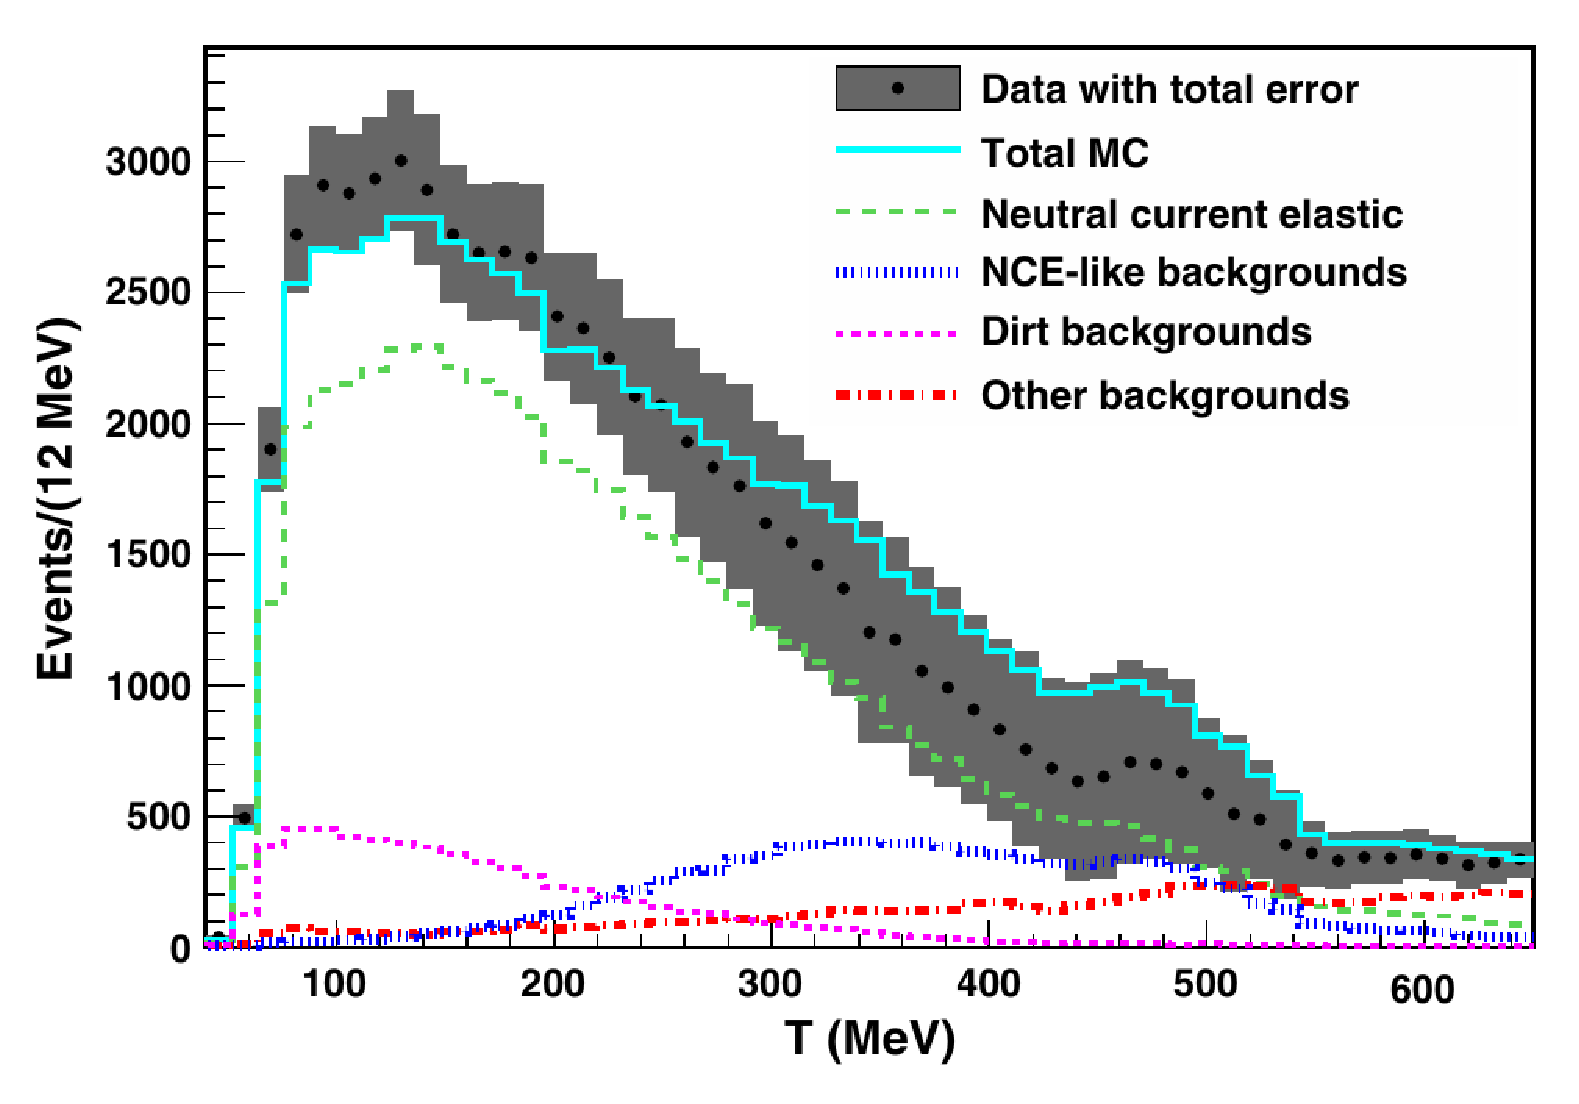
\includegraphics[width = \columnwidth]{img/mbnce1.eps}
    }
    {
      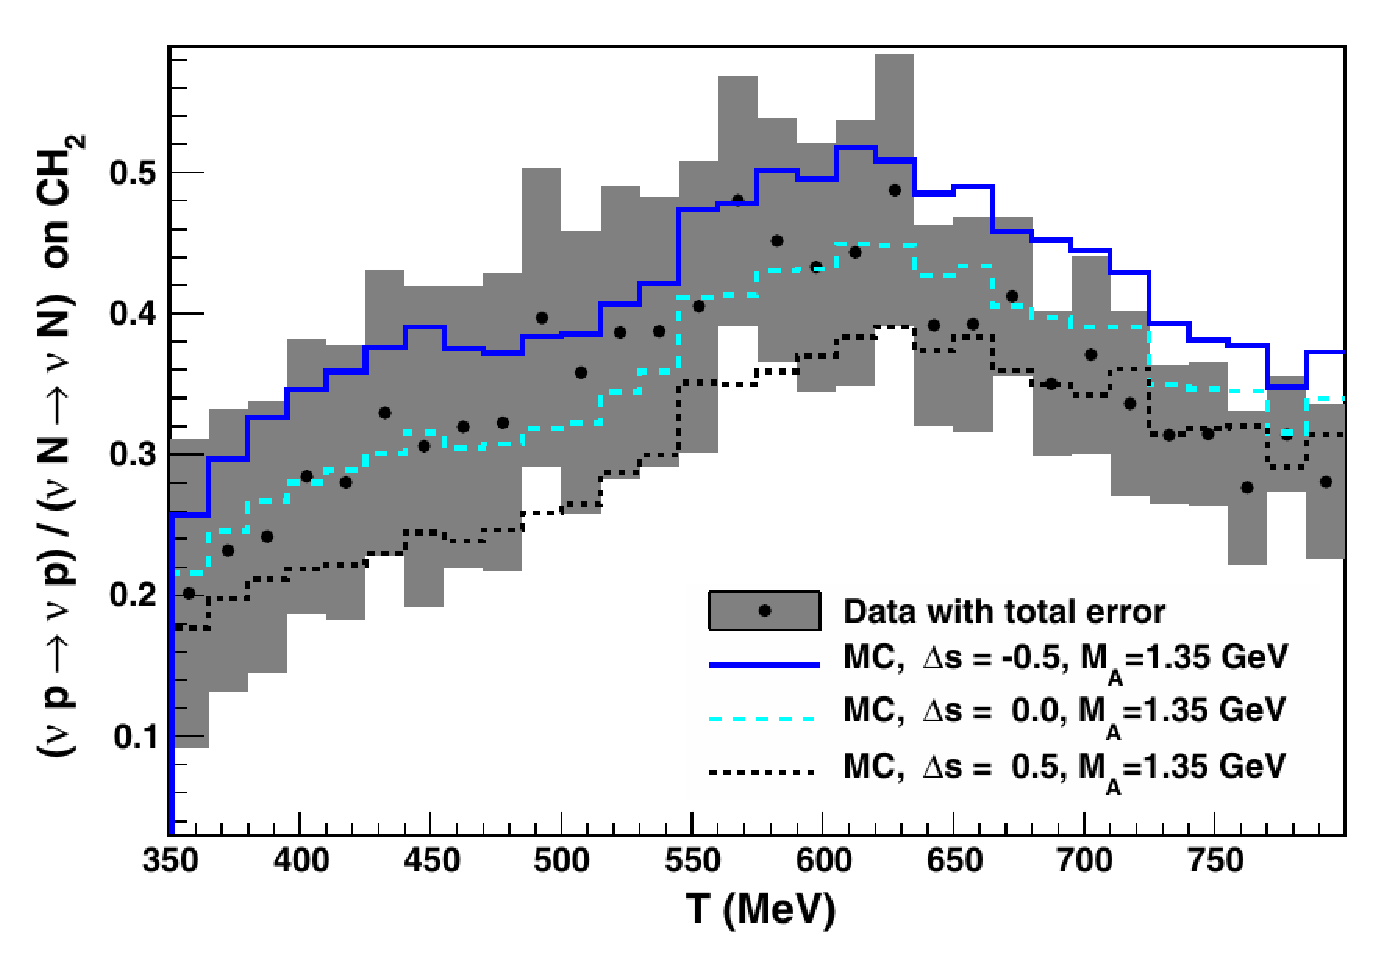
\includegraphics[width = \columnwidth]{img/mbnce2.eps}  
    }
    \vspace{10pt}
    {\centering\color{pdcolor4}\footnotesize $T$ stands for the total reconstructed energy of all nucleons in the final state.\\}
    \vspace{10pt}
    \twocolumn
    {
      \begin{itemize}
      
      \item Here assume $g_A^s = 0$.
      
      \item Best fit for: $$M_A = 1.39 \pm 0.11\mbox{~GeV}$$
      
      \vspace{-10pt}\item Inconsistency with older measurements $M_A \sim 1$~GeV.
      
      \end{itemize}
    }
    {

      \begin{itemize}
      
      \item Here assume {\footnotesize $M_A = 1.35$~GeV}.
      
      \item Best fit for: $$g_A^s = 0.08 \pm 0.26$$
      
      \vspace{-10pt}\item ``$\nu p \rightarrow \nu p$'' stands for events with proton above Cherenkov treshold.
      
      \end{itemize}
    }
  }
    
\end{slide}

%%%%% 2p2h %%%%%

\begin{wideslide}[toc=$np-nh$]{Two body current (or $np-nh$) contribution}
 
  \rput(16.5,4){% 2p2h 
\begin{pspicture}
  
  \psline[linewidth = 0.025, linecolor = pdcolor4]{->}(-1.2,0)(-0.65,0)
  
  \psline[linewidth = 0.025, linecolor = pdcolor1]{->}(0.1,0.2)(1.5,0.5)
  \psline[linewidth = 0.025, linecolor = pdcolor1]{->}(-0.1,-0.47)(1.25,-1.25)

  \pscircle[linewidth = 0.05, linecolor = pdcolor1](0,0){1}
  \pscircle[linestyle = none, fillstyle = solid, fillcolor = pdcolor1](-0.2, 0.2){0.2}
  \pscircle[linestyle = none, fillstyle = solid, fillcolor = pdcolor1](-0.4, -0.3){0.2}
  \pscircle[linestyle = none, fillstyle = solid, fillcolor = pdcolor1](0.3, 0.6){0.2}
  \pscircle[linestyle = none, fillstyle = solid, fillcolor = pdcolor1](0.4, -0.2){0.2}
  
  \rput[c]{70}(-0.3,-0.05){\psellipse[linewidth = 0.05, linecolor = pdcolor4](0,0)(0.6,0.4)}

  \pscircle[linestyle = none, fillstyle = solid, fillcolor = pdcolor4](-1.5, 0){0.2}
  
  
\end{pspicture}
}
  
  \begin{itemize}
   
   \item The $np-nh$ interactions occur on at least two nucleons.
   
   \item What is the isospin correlation?
   
   \item There are no new particles created, so the final state looks \\ the same as in elastic scattering.
   
   \item $np-nh$ is not taken into account in MiniBooNE analysis, which may cause the discrepancy with previous measurements of axial mass.
      
   \item There are two theoretical models of $np-nh$ (IFIC, Lyon), which take care about proper energy transfer distribution. Unfortunately, both are available only for CC channel.
   
   \item The phenomenological Transverse Enhancement (TE) model is used in the calculation. The $np-nh$ contribution is introduced by the modification of the vector magnetic form factors. Lepton kinematics is the same as for elastic scattering.
  
   \item The goal is to repeat the analysis with the inclusion if the $np-nh$ contribution.
  
  \end{itemize}

\end{wideslide}


%%%%% NUWRO ANALYSIS %%%%%

\begin{wideslide}[toc=Results with $np-nh$]{Simultaneous extraction of $M_A$ and $g_A^s$}
 
 \rput[c](11,-4.1){\includegraphics[width = 0.35\slidewidth]{img/kontur.eps}}
 \rput[c](4,-2.375){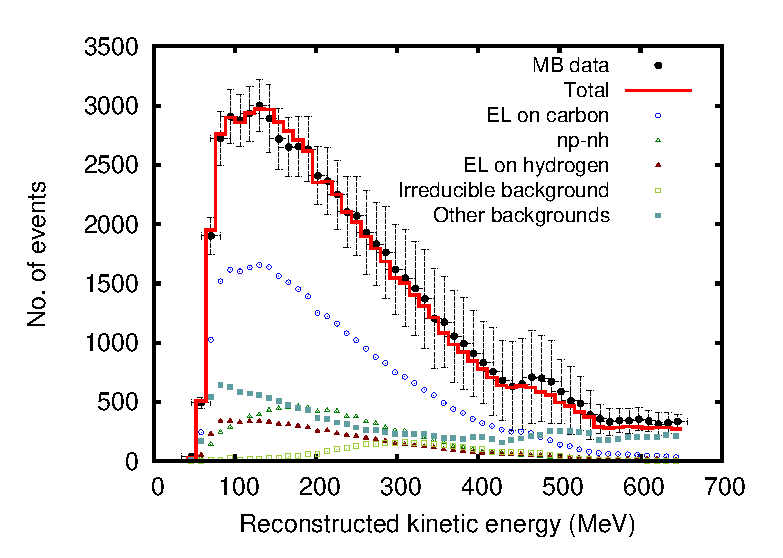
\includegraphics[width = 0.5\slidewidth]{img/bestfit.eps}}
 
 \vspace{155pt}
  
  \def\arraystretch{1.5}
  \hspace{22.5pt}\begin{tabular}{c || c | c}
    & w/o $np-nh$ & with $np-nh$ \\ \hline\hline
    $M_A$~{\tiny[GeV]} & $1.34^{+0.18}_{-0.10}$ & $1.10^{+0.13}_{-0.15}$ \\ \hline
    $g_A^s$ & $-0.5^{+0.2}_{-0.2}$ & $-0.4^{+0.5}_{-0.3}$
  \end{tabular}
  \vspace{15pt}\\
  {\color{pdcolor1}\small\bf Golan, Graczyk, Juszczak, Sobczyk PRC86 (2013) 024612}
  \rput[c](3,-0.1){\color{pdcolor3}\it made in Mathematica}
\end{wideslide}

\begin{slide}{The ratio issue}

  \rput[c](7.5,-2){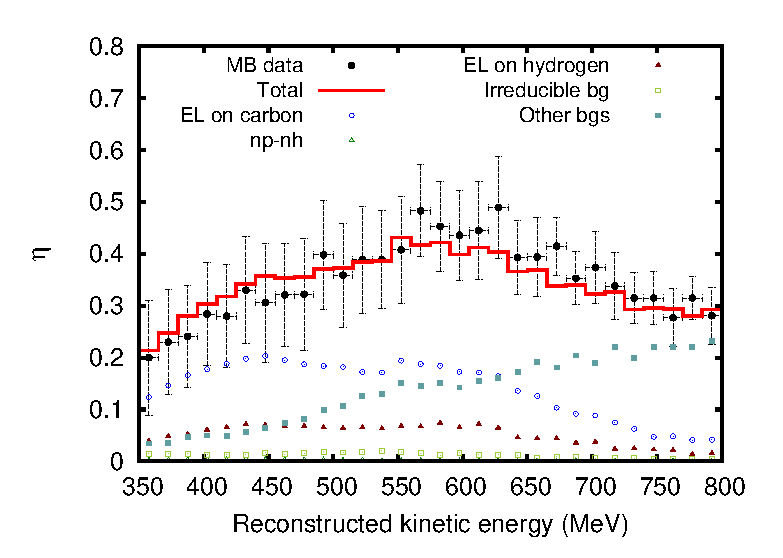
\includegraphics[width = 0.4\slidewidth]{img/ds_bestfit.eps}}

  \begin{itemize}

    \item The plot is made \\ using best fit values \\ from the last slide.
    
    \item It turns out that the ratio \\ is very sensitive \\ on the energy transfer \\ distribution (No. of \\ protons above threshold).
    
    \item The Transverse Enhancement does not take care properly of lepton kinematics, which affects the energy distribution of final state nucleons. It is not a proper model to analyze this data.
    
    \item This data, however,  has a potential to discriminate between IFIC and Lyon models...
    
    \item ... when they appear for neutral current channel.
  
  \end{itemize}

\end{slide}
